\chapter{Data Collection}
\label{sec:Data_Collection}

The data collection portion of this project is immediately tasked with the following set of problems: spatial coincidence, temporal coincidence, and resolution. Given the asynchronous orbits of each satellite and the incompatible resolutions of NASA's SN-2 with its own IS-2, other avenues were explored to obtain precise SAR imaging. Particularly, the European Space Agency (ESA) offered the 

\section {SAR Imaging}


\begin{figure}
    \centering
    \subfigure[]{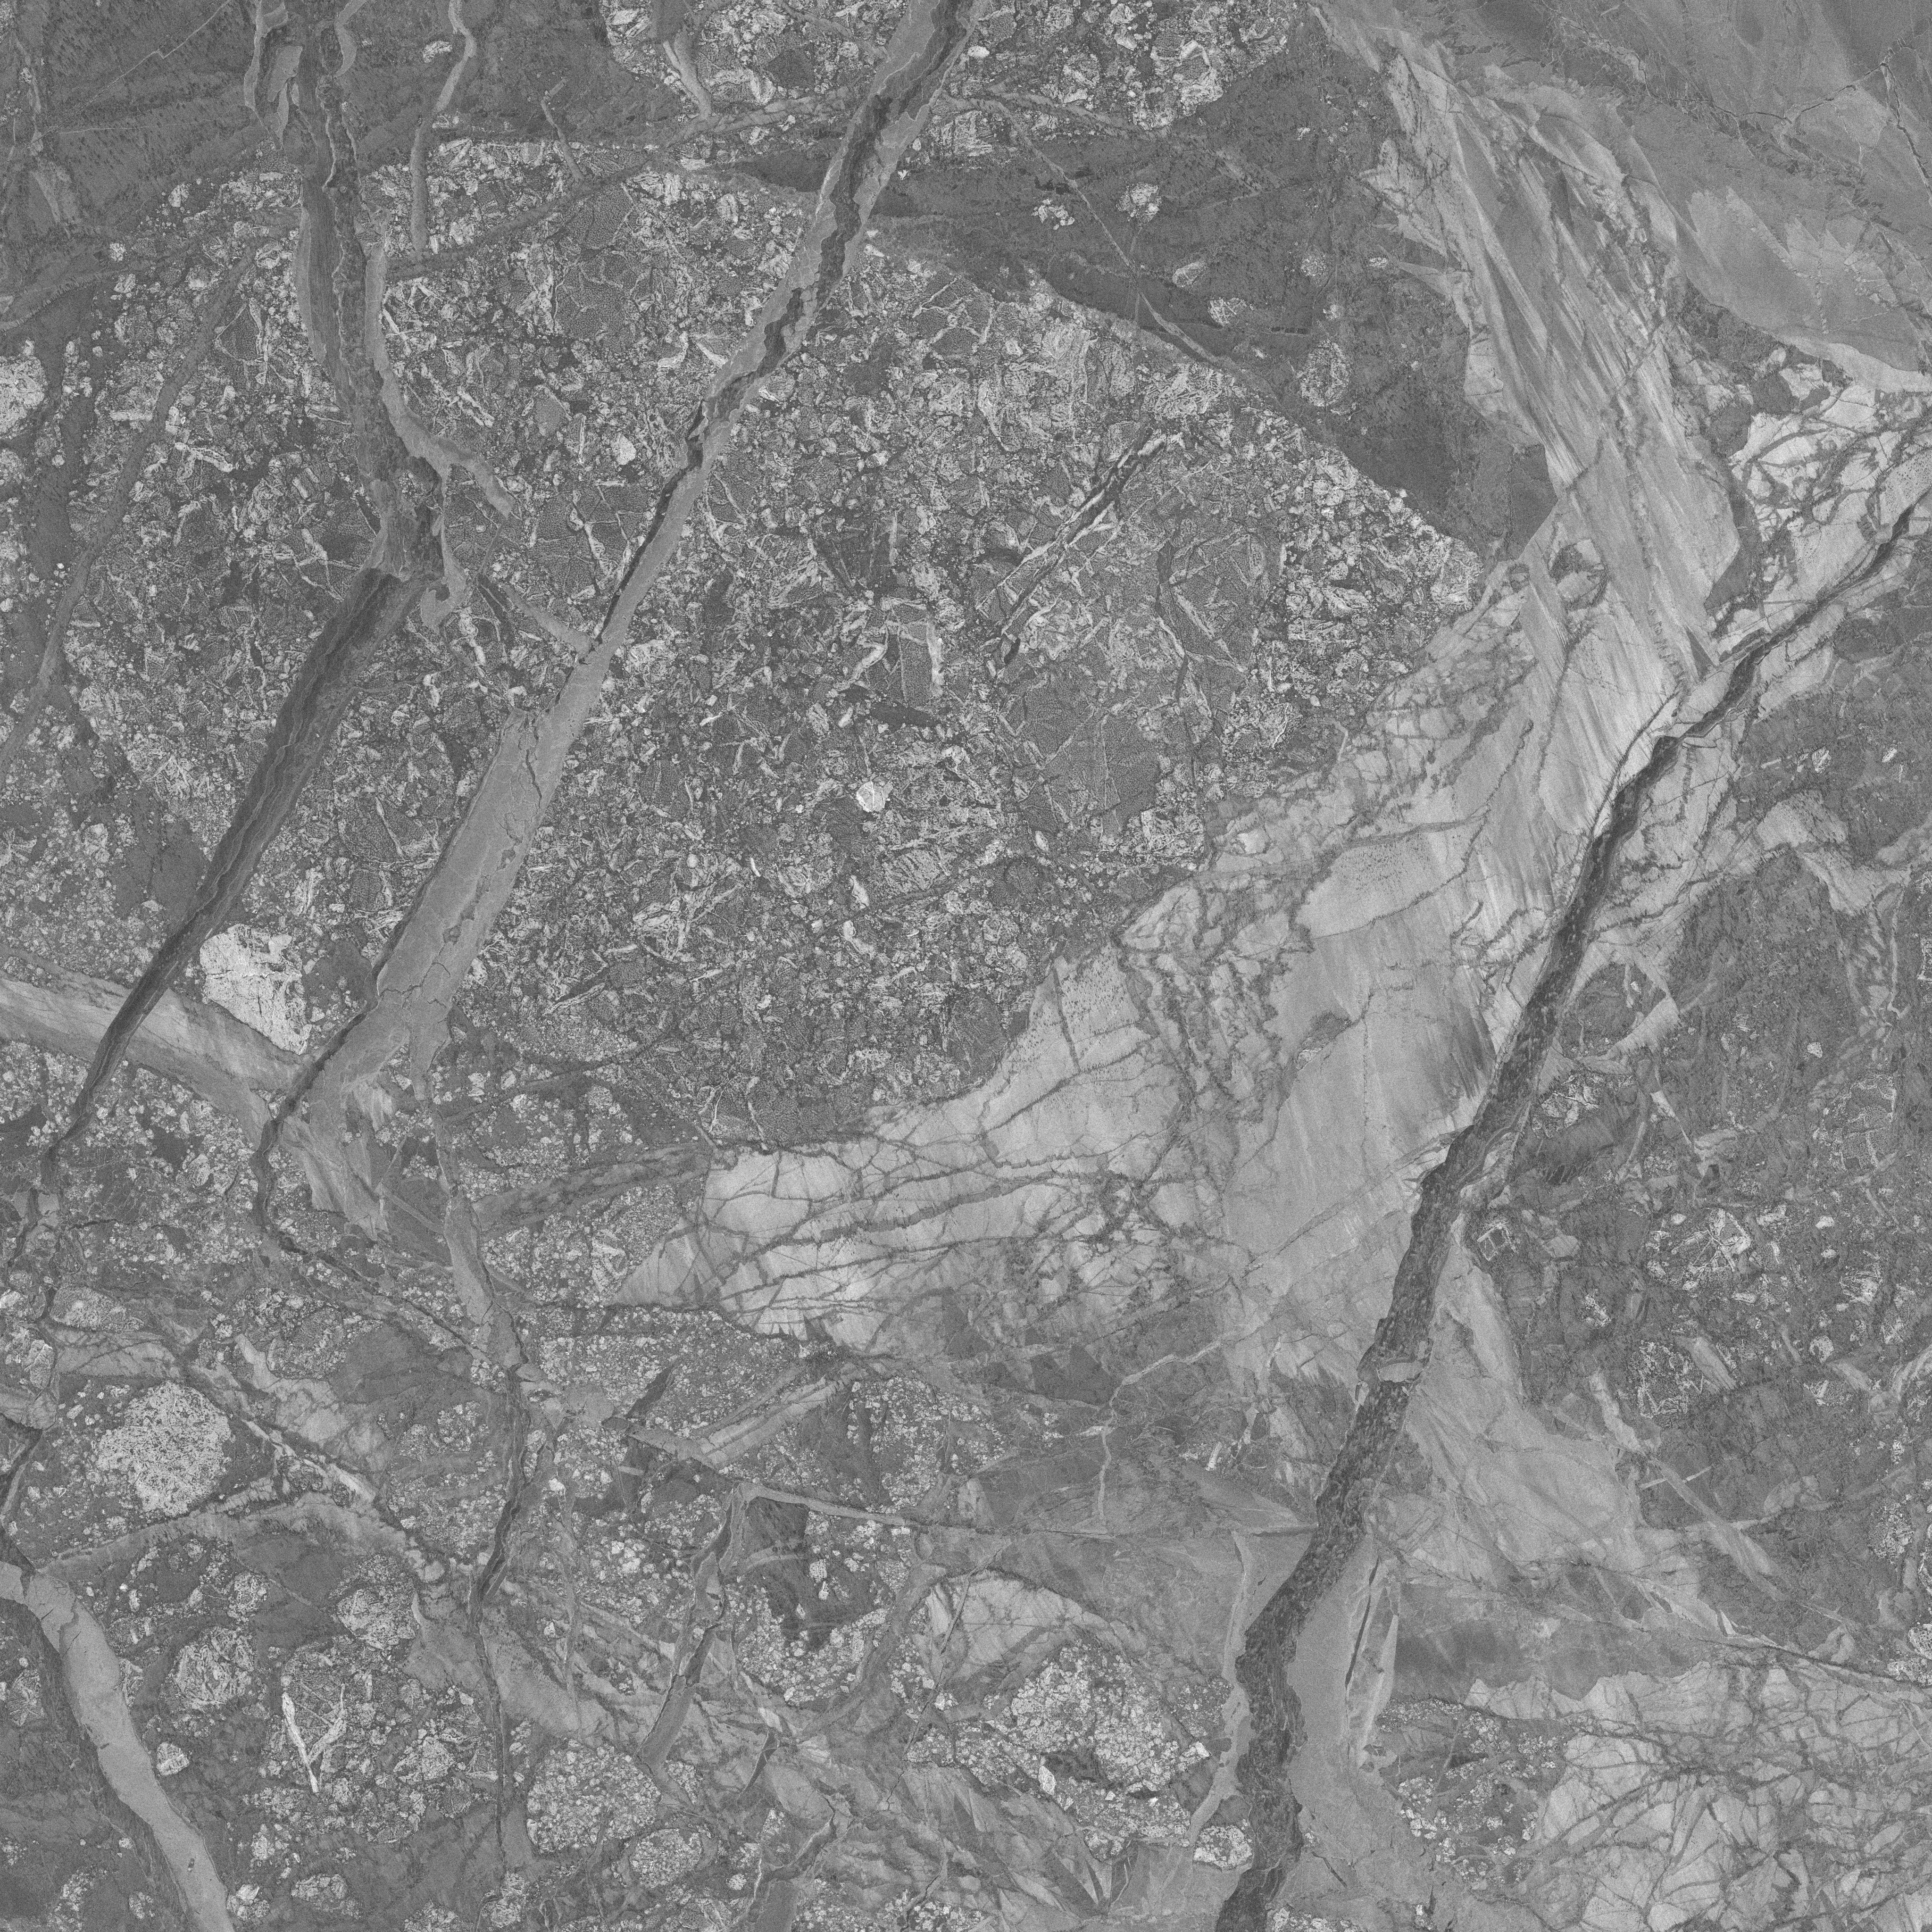
\includegraphics[width=.48\linewidth]{./research-resources/SAR/ICEYE_X2_QUICKLOOK_SLEA_3279211_20240119T044029.png}}
    \subfigure[]{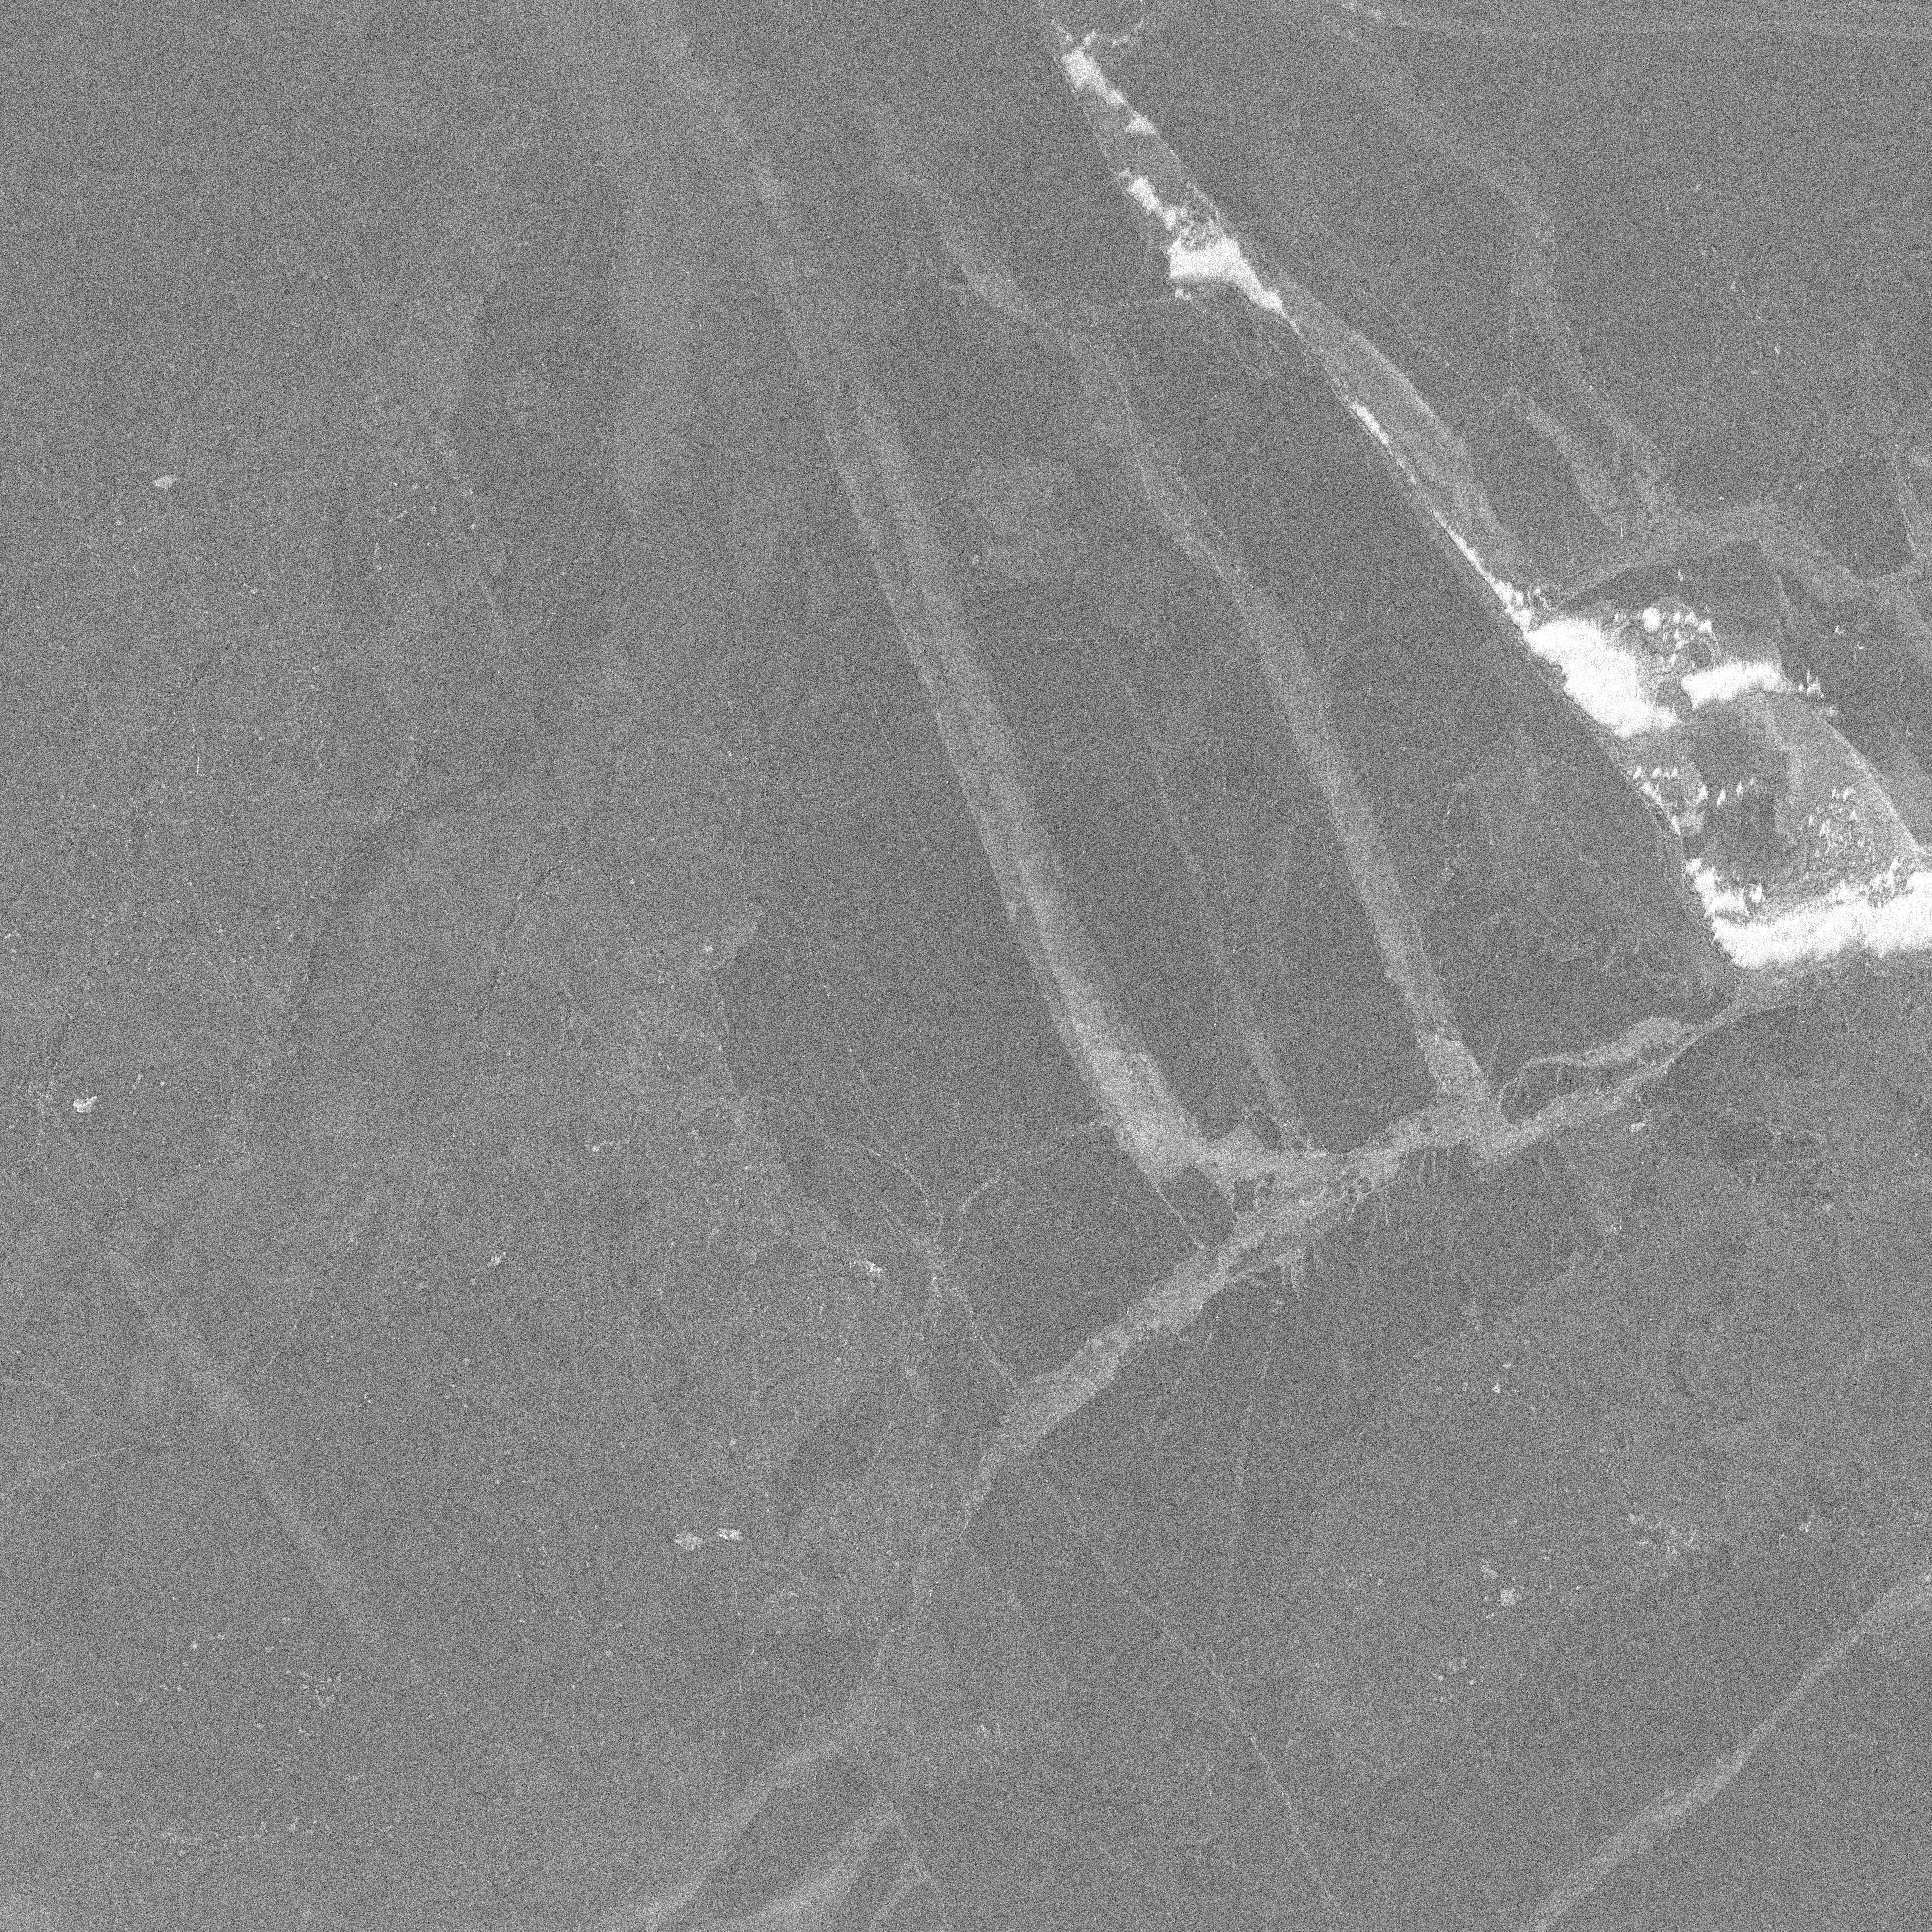
\includegraphics[width=.48\linewidth]{./research-resources/SAR/ICEYE_X6_QUICKLOOK_SLH_3280232_20240120T132858.png}}
    \subfigure[]{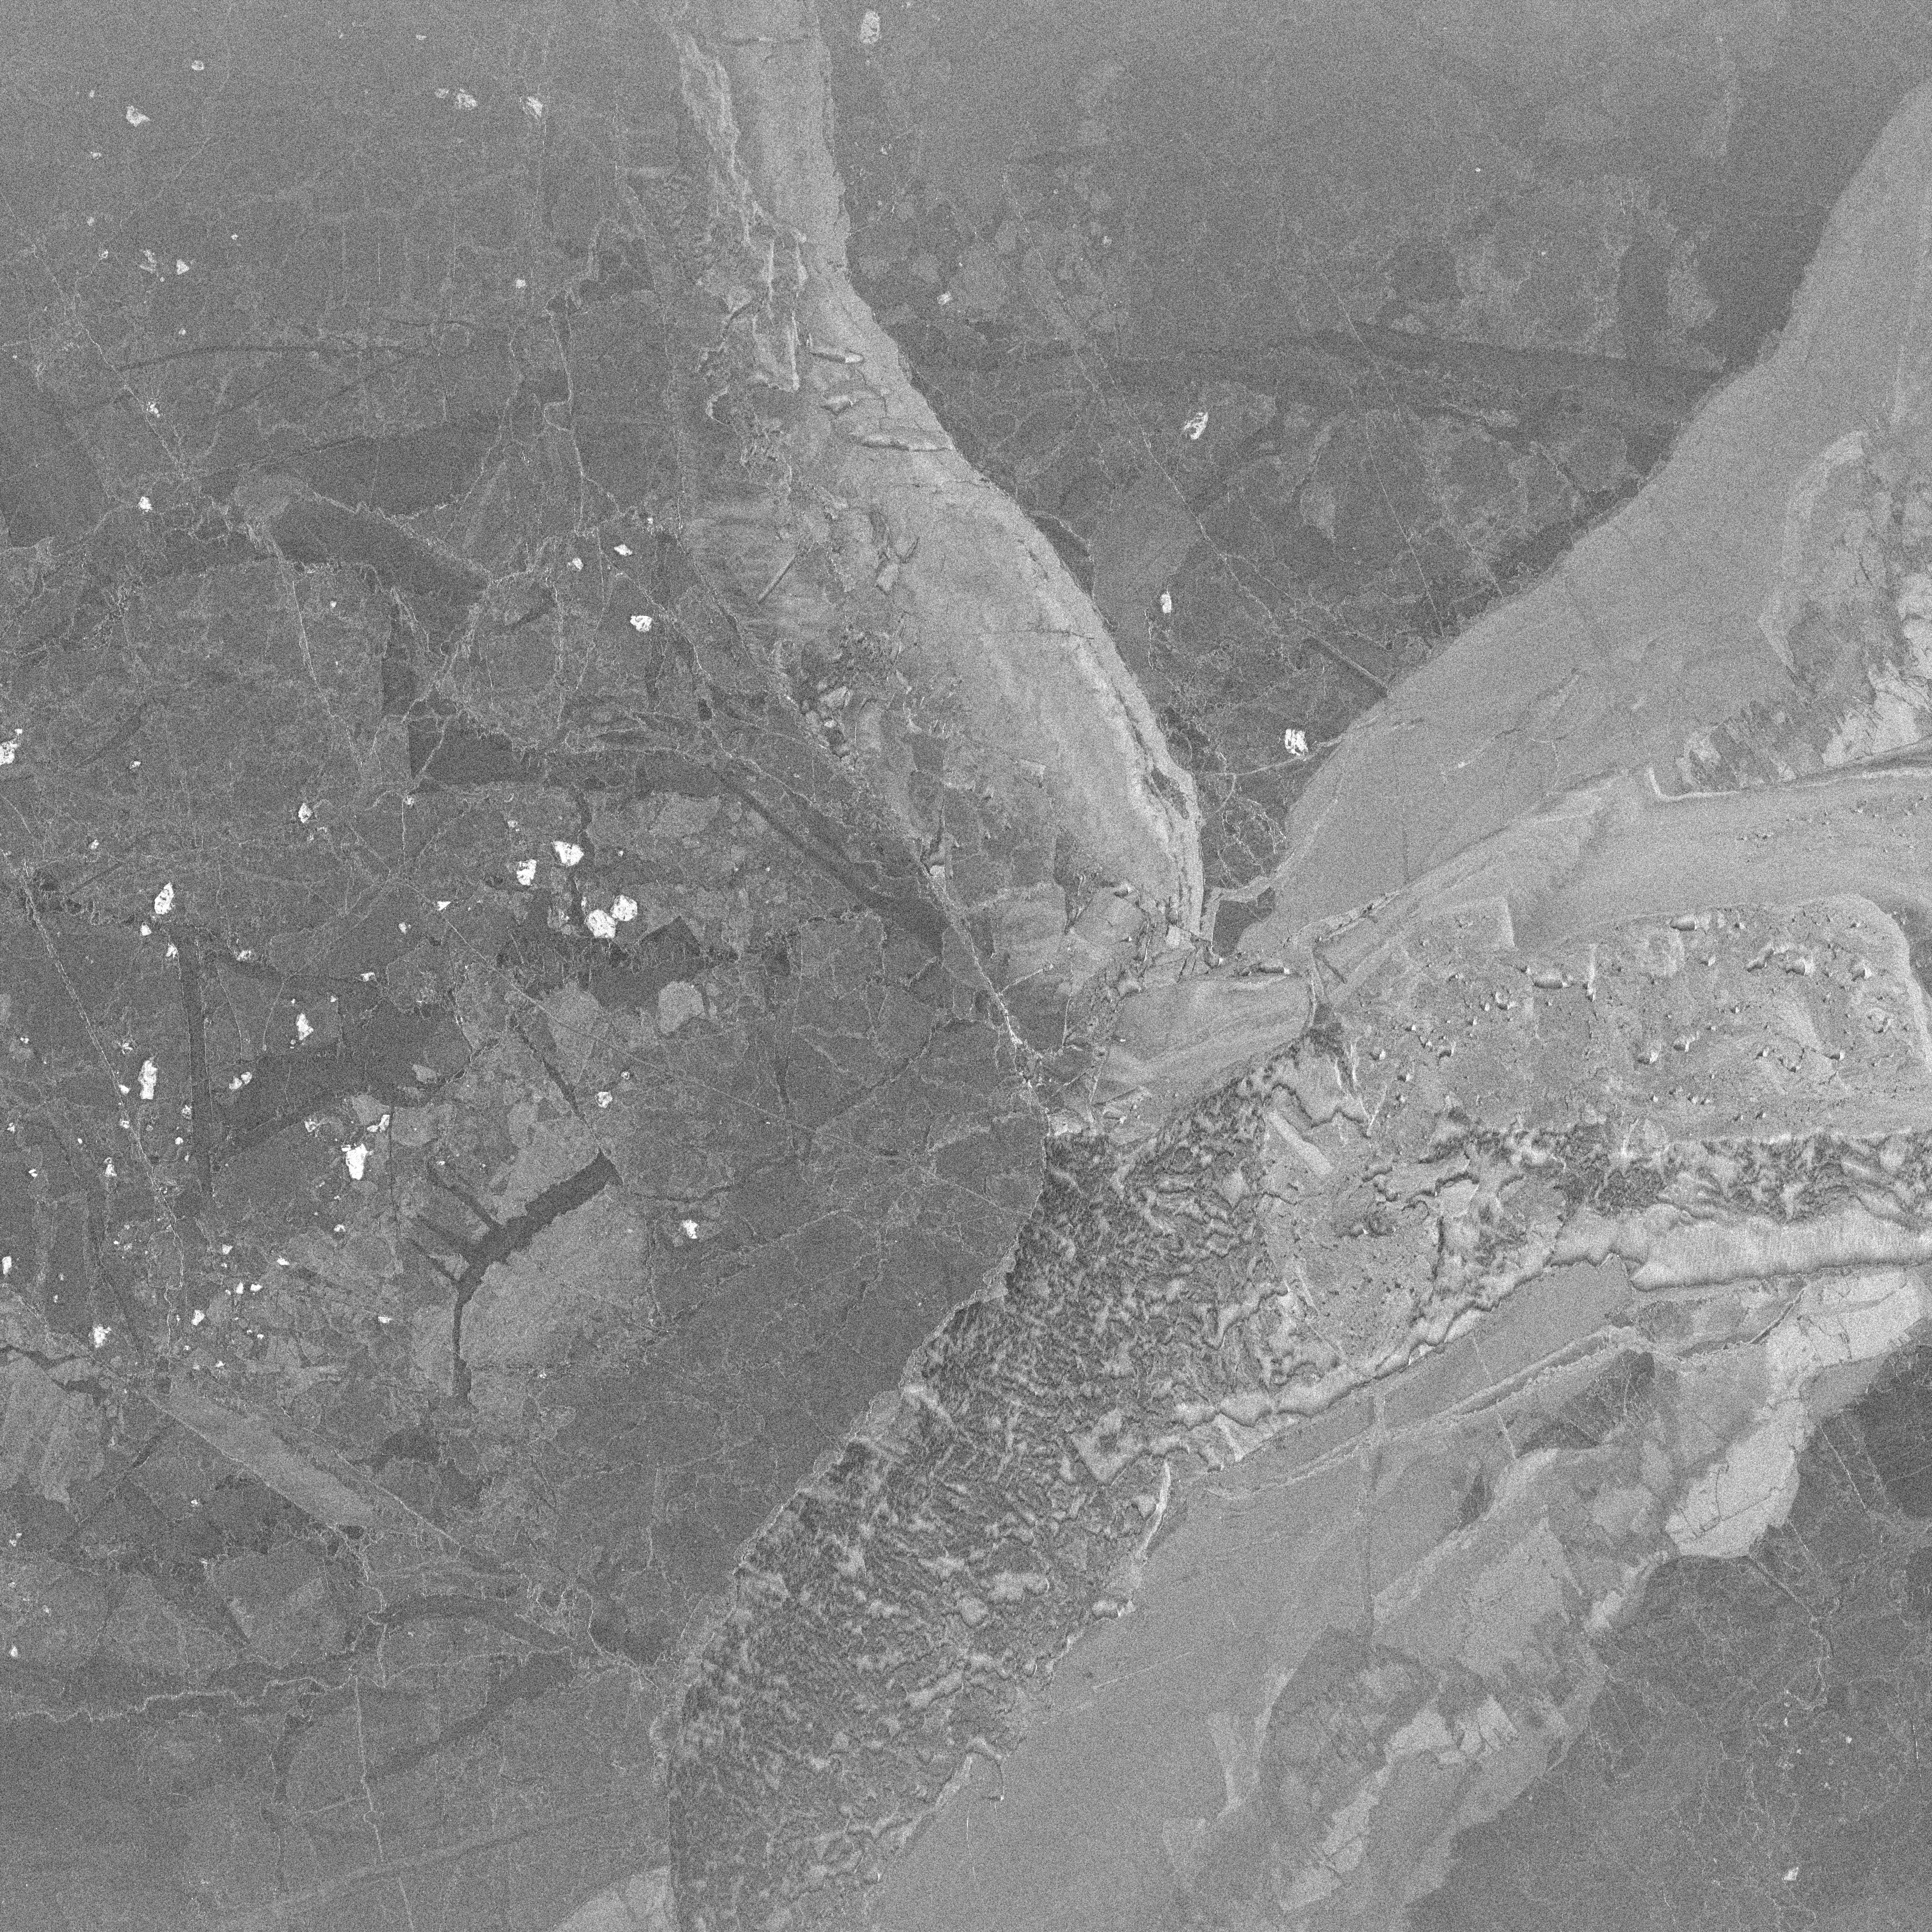
\includegraphics[width=.48\linewidth]{./research-resources/SAR/ICEYE_X8_QUICKLOOK_SLH_3295462_20240120T202547.png}}
    \subfigure[]{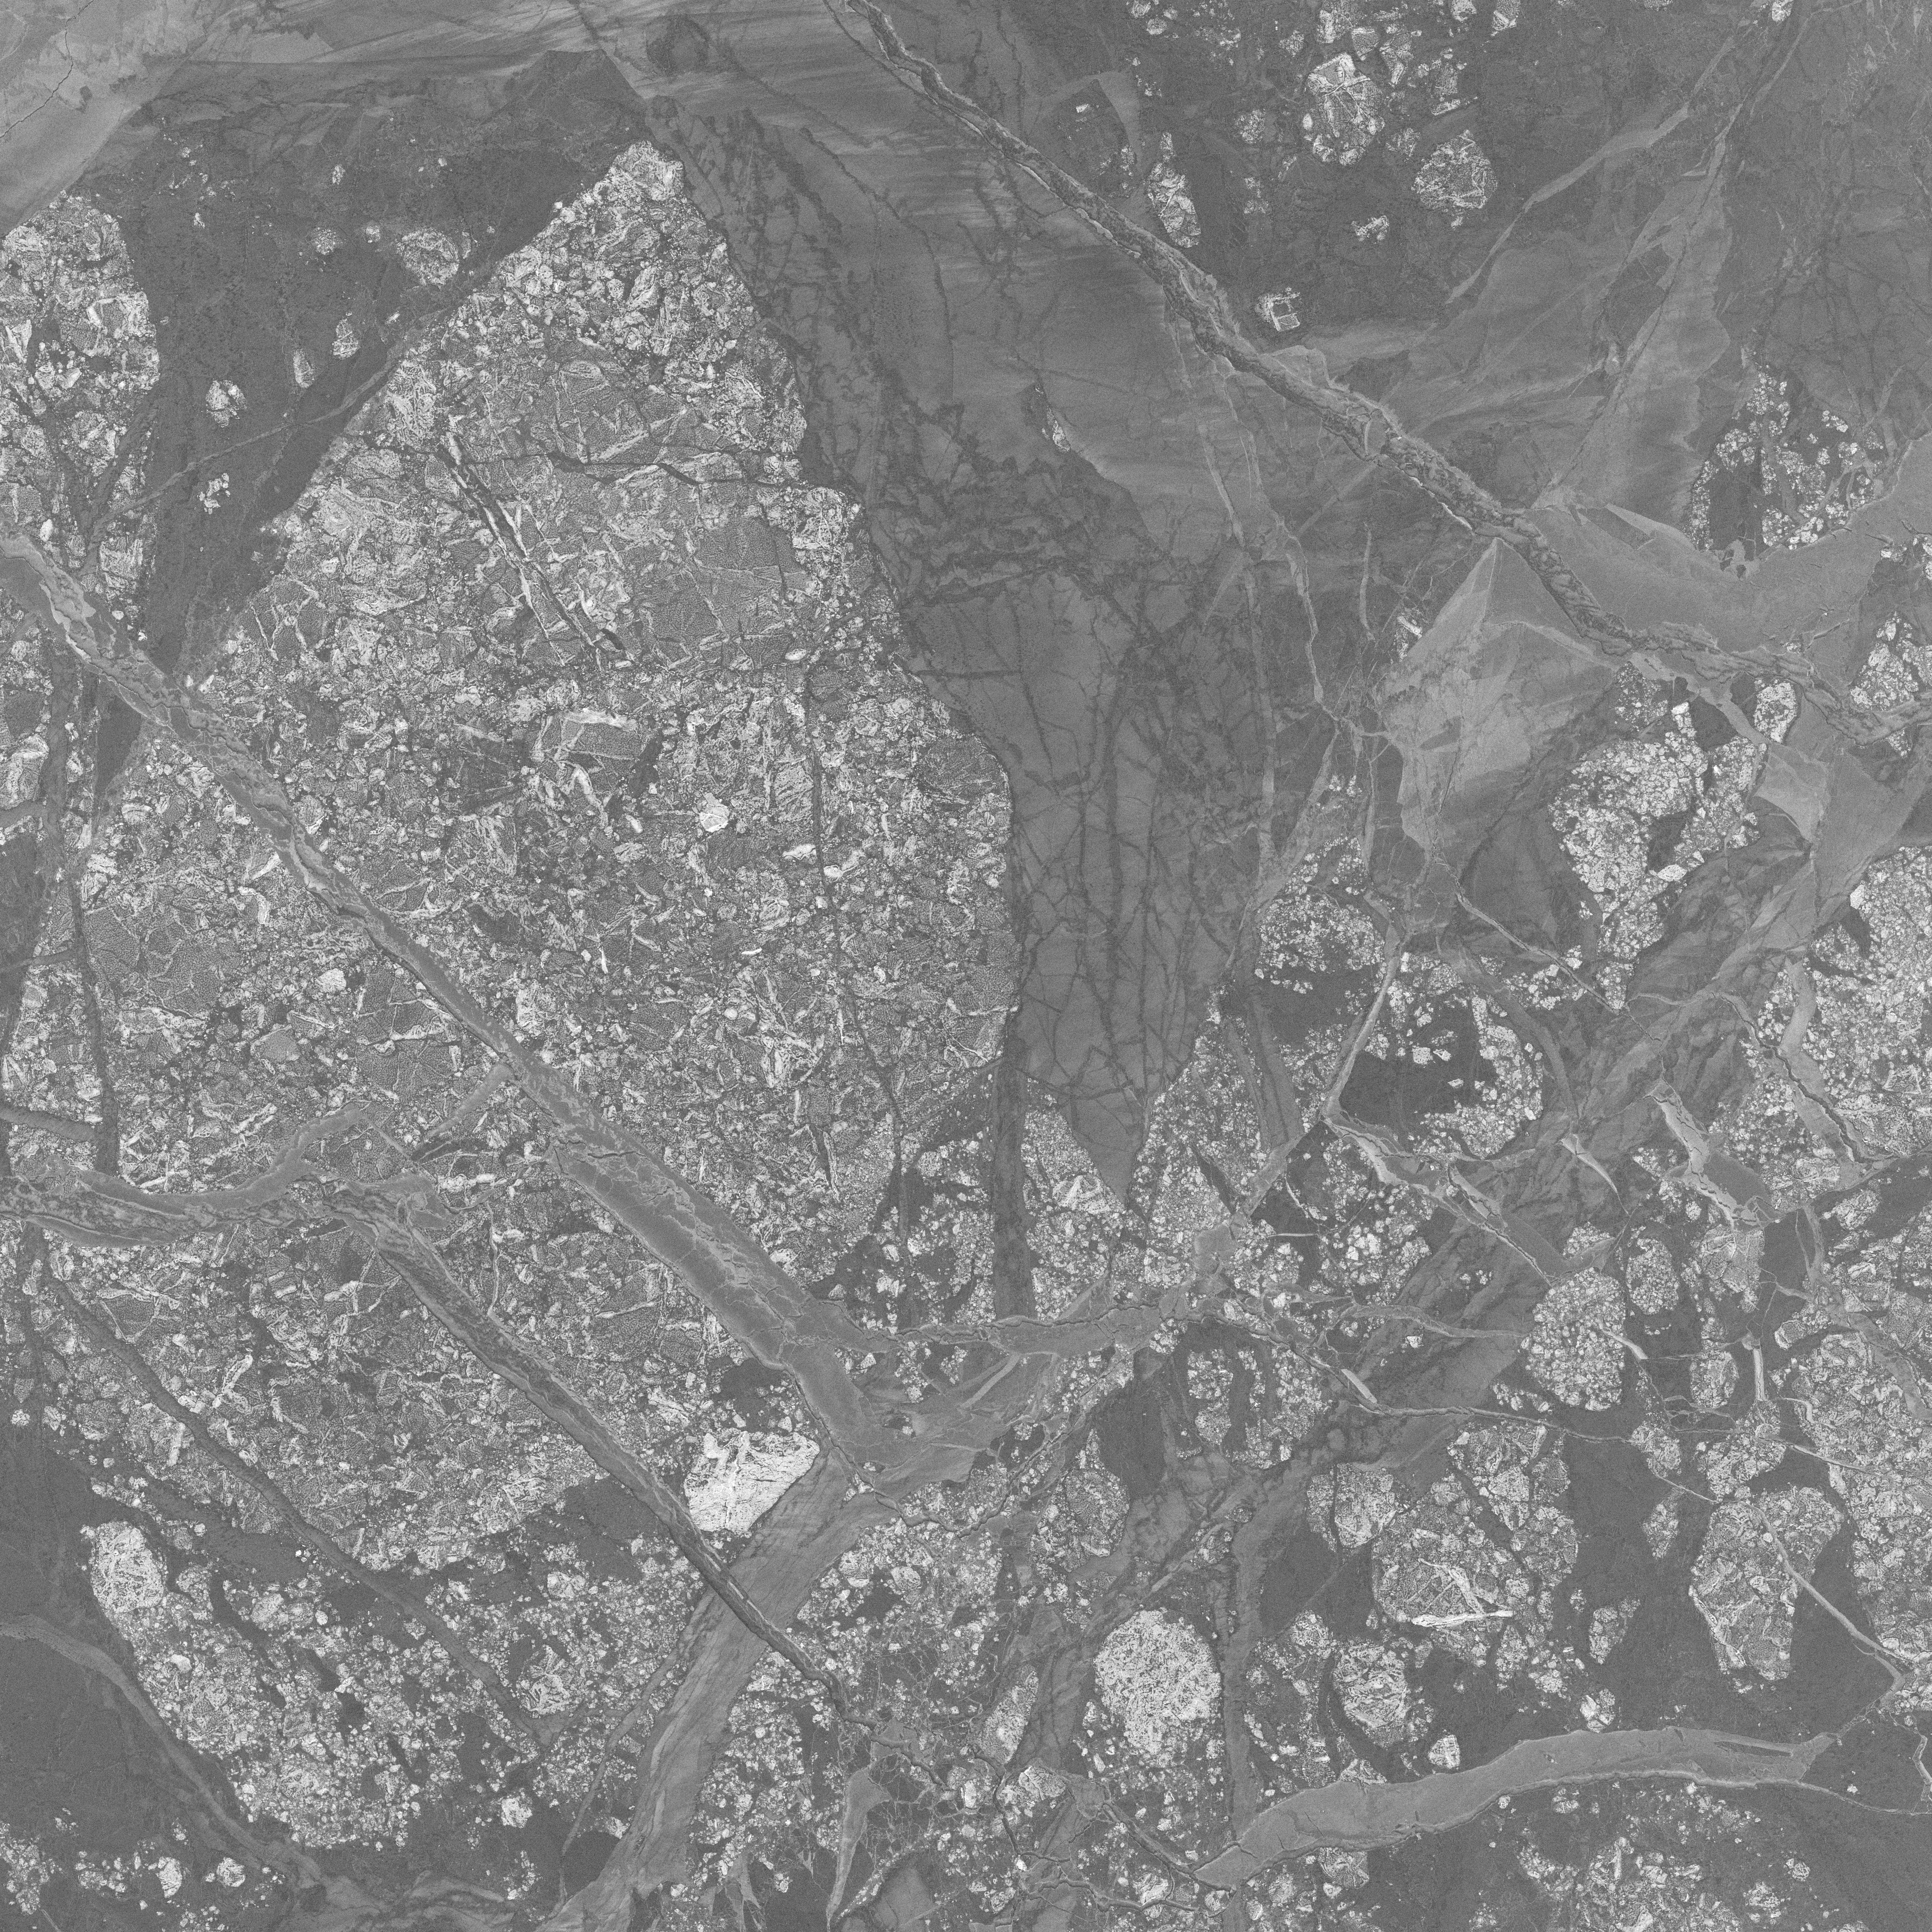
\includegraphics[width=.48\linewidth]{./research-resources/SAR/ICEYE_X13_QUICKLOOK_SLEA_3279210_20240119T023534.png}}
    \caption{(a), (b), (c), (d)}
    \label{gathered-sar}%
\end{figure}

\section {Laser Altimetry (IceSat-2)}



\begin{figure}[]
	\centering
	\includegraphics[width=.8\textwidth]{../research-resources/ice-sat-2/Surface Profiles.png}
	\caption{Ice Thicknesses}
	\label{fig:ice-thickness-gathered}
\end{figure}

------Default Text ----------

Provide in brief the background information for your work/field keeping in mind that maybe your readers do not have experience with topics your reference or address in your thesis. 

In the second part, provide a review of the state of the art relevant to your thesis. Here you present relevant research that relates to your work. 
